\documentclass[11pt,oneside,a4paper]{article}
\usepackage{graphicx}
\usepackage{booktabs}
\usepackage{caption}
\usepackage{subcaption}
\usepackage{amsmath}
\usepackage{amsfonts}
\usepackage{amssymb}
\usepackage{lscape}
\usepackage{psfrag}
\usepackage[usenames]{color}
\usepackage{bbm}
\usepackage[update]{epstopdf}
\usepackage[bookmarks,pdfstartview=FitH,a4paper,pdfborder={0 0 0}]{hyperref}
\usepackage{verbatim}
\usepackage{listings}
\usepackage{textcomp}
\usepackage{fancyhdr}
\usepackage{multirow}
\usepackage{tikz}
\usepackage{lipsum}
\usepackage{xcolor}
\usepackage{wrapfig}
\usepackage[margin=0.5in]{geometry}
\usepackage{pdfpages}
\usepackage[utf8]{inputenc}
\usepackage[compact]{titlesec}
\usepackage{paralist}
\newcommand{\hint}[1]{{\color{blue} \em #1}}

\makeatletter %% <- make @ usable in command names
\newcommand*\Neg[2][0mu]{\Neginternal{#1}{\negslash}{#2}}
\newcommand*\sNeg[2][0mu]{\Neginternal{#1}{\snegslash}{#2}}
\newcommand*\ssNeg[2][0mu]{\Neginternal{#1}{\ssnegslash}{#2}}
\newcommand*\sssNeg[2][0mu]{\Neginternal{#1}{\sssnegslash}{#2}}
\newcommand*\Neginternal[3]{\mathpalette\Neg@{{#1}{#2}{#3}}}
\newcommand*\Neg@[2]{\Neg@@{#1}#2}
\newcommand*\Neg@@[4]{%
	\mathrel{\ooalign{%
			$\m@th#1#4$\cr
			\hidewidth$\m@th#3{#1}\mkern\muexpr#2*2$\hidewidth\cr
	}}%
}

\newcommand*\negslash[1]{\m@th#1\not\mathrel{\phantom{=}}}
\newcommand*\snegslash[1]{\rotatebox[origin=c]{60}{$\m@th#1-$}}
\newcommand*\ssnegslash[1]{\rotatebox[origin=c]{60}{$\m@th#1{\dabar@}\mkern-7mu{\dabar@}$}}
\newcommand*\sssnegslash[1]{\rotatebox[origin=c]{60}{$\m@th#1\dabar@$}}
\makeatother  %% <- revert @

\makeatletter
\def\cleardoublepage{\clearpage\if@twoside \ifodd\c@page\else%
\hbox{}%
\thispagestyle{empty}%
\clearpage%
\if@twocolumn\hbox{}\clearpage\fi\fi\fi}
\makeatother

\sloppy
% \widowpenalty=10000
% \clubpenalty=10000

\title{
    \vspace*{0.0mm}
    \LARGE\bf\sf Big Data for Engineers (Spring 2020)
    \vspace*{10.0mm} \\
    %
    \Huge\bf\sf Summary
    %
    \vspace*{30.0mm} \\
    \normalsize
    %
    \sf Author:\\[5pt]
    \sf Yannick Merkli\\ [5pt]
    \sf \pageref{lastpage} Pages
}
\date{}

\begin{document}

\maketitle
\thispagestyle{empty}
\raggedbottom
\clearpage

\pagenumbering{roman}

\clearpage
\setcounter{tocdepth}{2}
\tableofcontents
\clearpage
\pagenumbering{arabic}

\setlength\parindent{0pt}
\titlespacing{\subsection}{0pt}{2ex}{2ex}


\newpage

\section{Introduction}

\subsection{History}

Databases have always existed in some way as a way to preserve information. It started with speaking and singing, went on with stone engraving and printing. Even before computers, tables were the primary format to represent data. Things changed drastically with the introduction of computers. Database management systems (DBMS) started with file systems (1960s), then we entered the relational era (1970s) and finally progressed into the NoSQL era (2000s) with the upcoming of big data.

\subsection{Big Data}

Big Data is a buzzword that goes across many disciplines (distributed systems, high-performance computing, data management, algorithms, statistics, machine learning, etc.) and that involves a lot of proprietary technology (AWS, Google Cloud, Microsoft Azure, etc.) which is simply a result of the need of companies to have efficient data systems.

The big in big data: \textbf{three Vs}

\vspace{-\topsep}
\begin{itemize}
	\setlength{\itemsep}{0pt}
	\setlength{\parskip}{0pt}
	\item Volume: Nowadays we have lots of sources of data (web, sensors, proprietary, scientific). Storage has become so cheap that we often just store data because we can. Further, data carries value; data is worth more than the sum of its parts (data totality: one must have complete data).
	\item Variety: We have different \textbf{data shapes}: tables, trees, graphs, cubes, text.
	\item Velocity: Data is generated automatically, Data is a realtime byproduct of human activity
\end{itemize}

\textbf{Prefixes (International System of Units)}

\begin{tabular}{|c|r|c|r|}
	\hline 
	kilo (k) & 1,000 (3 zeros) & kibi (ki) & 1,024 ($2^{10}$) \\ 
	\hline 
	Mega (M) & 1,000,000 (6 zeros) & Mebi (Mi) & 1,048,576 ($2^{20}$) \\ 
	\hline 
	Giga (G) & 1,000,000,000 (9 zeros) & Gibi (Gi) & 1,073,741,824 ($2^{30}$) \\ 
	\hline 
	Tera (T) & 1,000,000,000,000 (12 zeros) & Tebi (Ti) & 1,099,511,627,776 ($2^{40}$) \\ 
	\hline 
	Peta (P) & 1,000,000,000,000,000 (15 zeros) & Pebi (Pi) & 1,125,899,906,842,624 ($2^{50}$) \\ 
	\hline 
	Exa (E) & 1,000,000,000,000,000,000 (18 zeros) & Exbi (Ei) & 1,152,921,504,606,846,976 ($2^{60}$) \\ 
	\hline 
	Zetta (Z) & 1,000,000,000,000,000,000,000 (21 zeros) & Zebi (Zi) & 1,180,591,620,717,411,303,424 ($2^{70}$) \\ 
	\hline 
	Yotta (Y) & 1,000,000,000,000,000,000,000,000 (24 zeros) & Yobi (Yi) & 1,208,925,819,614,629,174,706,176 ($2^{80}$) \\ 
	\hline
\end{tabular}\newline

There are three paramount factors to big data:

\vspace{-\topsep}
\begin{itemize}
	\setlength{\itemsep}{0pt}
	\setlength{\parskip}{0pt}
	\item Capacity: "How much data can we store?"
	\item Throughput: "How fast can we transmit data?"
	\item Latency: "When do I start receiving data?"
\end{itemize}
\vspace{-\topsep}

Capacity has improved incredibly much over the past 60 years (1956: huge HDD had 5MB storage, 2020: there are palm sized 20TB HDDs). Capacity has increased by a factor $200 * 10^9$ (per unit of volume). However, throughput and latency have only improved by a factor $10'000$ and $200$ respectively. This discrepancy creates problems: the throughput no longer scales to the amount of data and the latency no longer scales to the throughput. Solution:

\vspace{-\topsep}
\begin{itemize}
	\setlength{\itemsep}{0pt}
	\setlength{\parskip}{0pt}
	\item Capacity-throughput discrepancy: parallelization
	\item Throughput-latency discrepancy: batch processing
\end{itemize}
\vspace{-\topsep}

\textbf{What is big data?}

Big Data is a portfolio of technologies that were designed to store, manage and analyze data that is too large to fit on a single machine while accommodating for the issue of growing discrepancy between
capacity, throughput and latency.

\section{Lessons learnt from the past}

\textbf{Data Independence:}\\
An underlying principle that has been valid for a long time is the principle of \textbf{data independence} (developed by Edgar Codd): Data Independence is defined as a property of DBMS that helps you to change the Database schema at one level of a database system without requiring to change the schema at the next higher level. Data independence helps you to keep data separated from all programs that make use of it.\\
This means we could e.g. change the physical storage (e.g. iPad instead of HDD) \textit{without} changing the logical data model.\\

\textbf{Overall architecture}\\
The overall architecture of a DBMS consists of:

\vspace{-\topsep}
\begin{itemize}
	\setlength{\itemsep}{0pt}
	\setlength{\parskip}{0pt}
	\item Language (e.g. SQL)
	\item Model (e.g. Tables (old); graphs, trees, cubes (new)
	\item Compute (e.g. single CPU (old); hadoop cluster (new))
	\item Storage (e.g. HDD (old); distributed storage (new)
\end{itemize}
\vspace{-\topsep}

A data model essentially describes \textit{what data looks like} and \textit{what you can do with the data}.

\subsection{Basic concepts}

\begin{itemize}
	\setlength{\itemsep}{0pt}
	\setlength{\parskip}{0pt}
	\item Table (Collection): A set of rows (= business object, item, entity, document, record) and each row has attributes (= columns)
	\item Attribute (column, field, property): A certain attribute of a row
	\item Primary key (row ID, name): a unique identifier of a row
\end{itemize}
\vspace{-\topsep}

\subsection{Relational Algebra}

We can look at tables as relations or as partial functions, mapping property to value\\
($f \in \mathbb{S} \ssNeg \rightarrow \mathbb{V}$), e.g. $city \mapsto Zurich$.

\subsubsection{Relations (the math, for database scientists)}

A relation R is made of:
\vspace{-\topsep}
\begin{itemize}
	\setlength{\itemsep}{0pt}
	\setlength{\parskip}{0pt}
	\item A set of attributes: $Attributes_R \subseteq \mathbb{S}$
	\item An extension (set of tuples): $$Extension_R \subseteq \mathbb{S} \ssNeg \rightarrow \mathbb{V} \quad s.t. \quad \forall t \in Extension_R, support(t) = Attributes_R$$
\end{itemize}
\vspace{-\topsep}

\textbf{Tabular integrity:} Holds if all rows have the same attributes and have a valid value for the attributes.\\
\textbf{Atomic integrity:} No tables in tables.\\
\textbf{Domain integrity:} All attribute values are of the specified type (e.g. an attribute \textit{Name} of type string can't be an integer).\\

In SQL, tabular integrity, atomic integrity and domain integrity all hold. In NoSQL however, none of these three properties hold.

\subsection{The relational model of data}

\begin{compactitem}
	\item Data Models: A data model is a notation for describing the structure of the data in a database, along with the constraints on that data. The data	model also normally provides a notation for describing operations on that data: queries and data modifications.
	\item Relational Model: Relations axe tables representing information. Columns are headed by attributes; each attribute has an associated domain, or	data type. Rows are called tuples, and a tuple has one component for each attribute of the relation.
	\item Schemas: A relation name, together with the attributes of that relation and their types, form the relation schema. A collection of relation schemas forms a database schema. Particular data for a relation or collection of relations is called an instance of that relation schema or database schema.
	\item Keys: An important type of constraint on relations is the assertion that an attribute or set of attributes forms a key for the relation. No two tuples of a relation can agree on all attributes of the key, although they can agree on some of the key attributes.
	\item Semistructured Data Model: In this model, data is organized in a tree or graph structure. XML is an important example of a semistructured data model.
	\item SQL: The language SQL is the principal query language for relational database systems. The current standard is called SQL-99. Commercial systems generally vary from this standard but adhere to much of it.
	\item Data Definition: SQL has statements to declare elements of a database schema. The CREATE TABLE statement allows us to declare the schema for stored relations (called tables), specifying the attributes, their types, default values, and keys.
	\item Altering Schemas: We can change parts of the database schema with an ALTER statement. These changes include adding and removing attributes from relation schemas and changing the default value associated with an attribute. We may also use a DROP statement to completely eliminate relations or other schema elements.
	\item Relational Algebra: This algebra underlies most query languages for the relational model. Its principal operators are union, intersection, difference, selection, projection, Cartesian product, natural join, theta-join, and renaming.
	\item Selection and Projection: The selection operator produces a result consisting of all tuples of the argument relation that satisfy the selection condition. Projection removes undesired columns from the argument relation to produce the result.
	\item Joins: We join two relations by comparing tuples, one from each relation.	In a natural join, we splice together those pairs of tuples that agree on all attributes common to the two relations. In a theta-join, pairs of tuples are concatenated if they meet a selection condition associated with the theta-join.
	\item Constraints in Relational Algebra: Many common kinds of constraints can be expressed as the containment of one relational algebra expression in another, or as the equality of a relational algebra expression to the empty set.
\end{compactitem}

\subsection{Relational queries}

The following table shows the operators used in Relational Algebra.

\vspace{-\topsep}
\begin{figure}[hb]
	\centering
	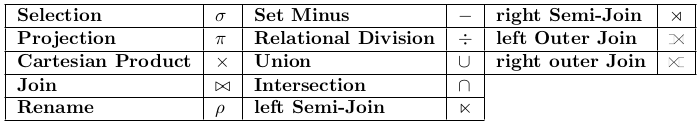
\includegraphics[width=0.7\linewidth]{figures/relational_algebra_operators}
	\label{fig:relationalalgebraoperators}
\end{figure}
\vspace{-\topsep}

\textbf{Projection:} The projection operator is used to produce from a relation R a new relation that has only some of R’s columns. The value of expression $\prod_{A_1,...,A_n}(R)$ is a relation that only
consists of columns for the attributes $A_1,...,A_n$.

\textbf{Selection:} The selection operator applied to R produces a new relation with a subset of R’s tuples, namely those who meet some condition C. This operation is denoted by $\sigma_C(R)$.

\textbf{Cartesian product:} The Cartesian product of relations R, S, denoted $R \times S$, simply concatenates every possible combination of tuples $r \in R, s \in S$. If R, S have attributes in common: rename them. In practice rarely used without join operators.

\textbf{Natural Join:} The natural join of relations L, R, denoted $L \bowtie R$, pairs only those tuples from L and R that agree in whatever attributes they share commonly. Natural Join is associative!
Other variants:

\vspace{-\topsep}
\begin{itemize}
	\setlength{\itemsep}{0pt}
	\setlength{\parskip}{0pt}
	\item Left outer join: natural join \& unmatched tuples from L
	\item Right outer join: natural join \& unmatched tuples from R
	\item Full outer join: natural join \& unmatched tuples from both L and R
	\item Left semi join: tuples from L that match with some tuple in R
	\item Right semi join: tuples from R that match with some tuple in L
\end{itemize}
\vspace{-\topsep}

\textbf{Theta-Join:} A theta join $\bowtie_\theta$ allows to join tuples from two relations R, S based on an arbitrary condition $\theta$ rather than solely based on attribute agreement. We get this new relation by:

\vspace{-\topsep}
\begin{enumerate}
	\setlength{\itemsep}{0pt}
	\setlength{\parskip}{0pt}
	\item Take the Cartesian product $R \times S$
	\item select those tuples satisfying condition $\theta$
\end{enumerate}
\vspace{-\topsep}

\textbf{Union, Intersection, Set Minus:} requires: both relations have the same schema $\rightarrow$ then consider set of tuples, do corresponding set operations. Note that $R \cap S = R - (R - S)$

\textbf{Rename:} 

\vspace{-\topsep}
\begin{itemize}
	\setlength{\itemsep}{0pt}
	\setlength{\parskip}{0pt}
	\item to change the name of the relation R to S, we write $\rho_S(R)$. 
	\item to rename attributes of R, we use the operator $\rho_{(A_1,..,A_n)}(R)$ where the attributes in the result relation S are called $A_1,...,A_n$, respectively.
\end{itemize}
\vspace{-\topsep}

\newpage

\subsection{Terminology}

Data: Data Manipulation Language (DML) (Query, insert, remove rows)
Schema: Data Definition Language (DDL) (Create or table/schema, drop it)
\vspace{-\topsep}
\begin{figure}[hb!]
	\centering
	\begin{subfigure}[t]{.5\textwidth}
		\centering
		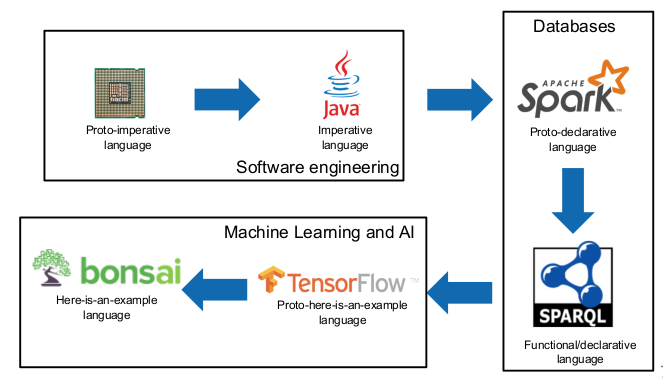
\includegraphics[width=0.8\linewidth]{figures/language_landscape}
		\caption{Language landscape}
		\label{fig:languagelandscape}
	\end{subfigure}%
	\begin{subfigure}[t]{.5\textwidth}
		\centering
		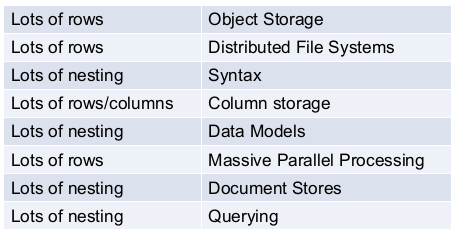
\includegraphics[width=0.8\linewidth]{figures/scaling_up_overview}
		\caption{Data Scale-Up}
		\label{fig:scalingupoverview}
	\end{subfigure}
\end{figure}

\subsection{Transactions}

The good old times of databases: ACID (Atomicity, Consistency, Isolation, Durability).

\vspace{-\topsep}
\begin{itemize}
	\setlength{\itemsep}{0pt}
	\setlength{\parskip}{0pt}
	\item Atomicity: Either the entire transaction is applied, or none of it (rollback).
	\item Consistency: After a transaction, the database is in a consistent state again.
	\item Isolation: A transaction feels like nobody else is writing to the database.
	\item Durability: Updates made do not disappear again.
\end{itemize}
\vspace{-\topsep}

\subsection{Performance}

Optimize for read vs. write intensive:
\vspace{-\topsep}
\begin{itemize}
	\setlength{\itemsep}{0pt}
	\setlength{\parskip}{0pt}
	\item OnLine Transaction Processing	(OLTP):	Write-intensive
	\item OnLine Analytical Processing (OLAP): Read-intensive
\end{itemize}

There is no such thing as "one size fits all" - data shape matters.

\subsection{Data scale-up}

Data can have lots of rows, lots of columns and lots of nesting. For the rest of this lecture, we are concerned with exactly this: scaling up!

\newpage

\titlespacing{\subsection}{0pt}{0ex}{0ex}

\section{SQL}

SQL is a family of standards, namely it includes a data definition language for schemas, a data manipulation language for updates and a query language for reads. Note that SQL is case-insensitive.

\subsection{DDL: Data Definition Language}
\vspace{-\topsep}
\begin{figure}[hb!]
	\centering
	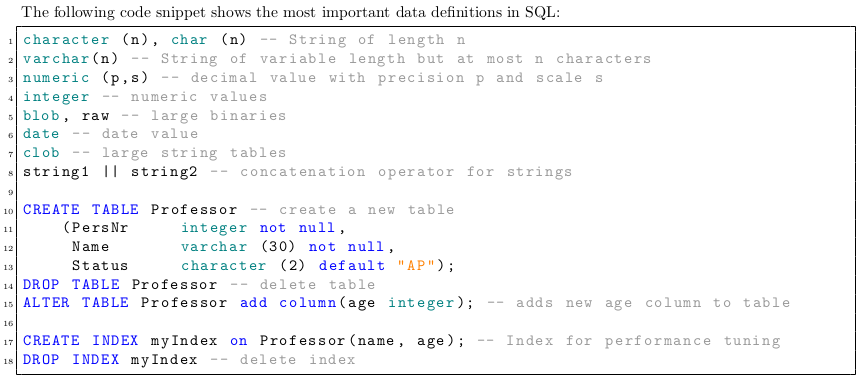
\includegraphics[width=1\linewidth]{figures/sql_1}
	\label{fig:sql1}
\end{figure}
\vspace{-\topsep}

\subsection{DML: Data Manipulation Language}
\vspace{-\topsep}
\begin{figure}[hb!]
	\centering
	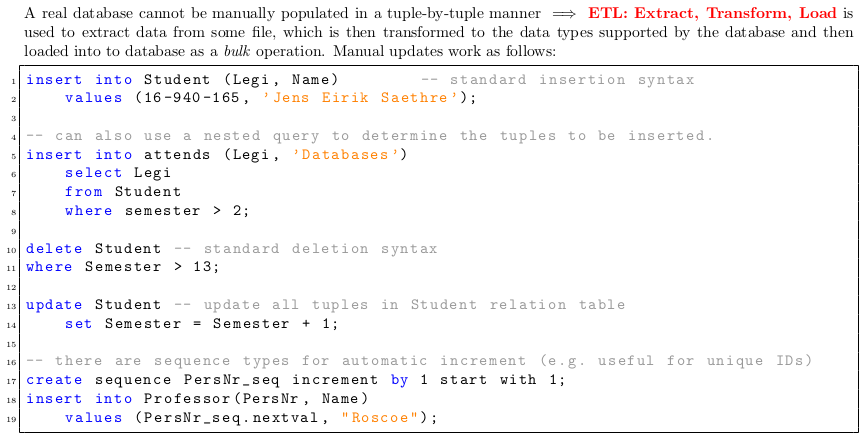
\includegraphics[width=1\linewidth]{figures/sql_2}
	\label{fig:sql2}
\end{figure}
\vspace{-\topsep}

\subsection{Simple Queries in SQL}
\vspace{-\topsep}
\begin{figure}[hb!]
	\centering
	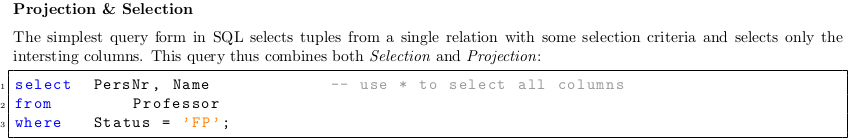
\includegraphics[width=1\linewidth]{figures/sql_3}
	\label{fig:sql3}
\end{figure}
\vspace{-\topsep}

\newpage
\vspace{-\topsep}
\begin{figure}[t!]
	\centering
	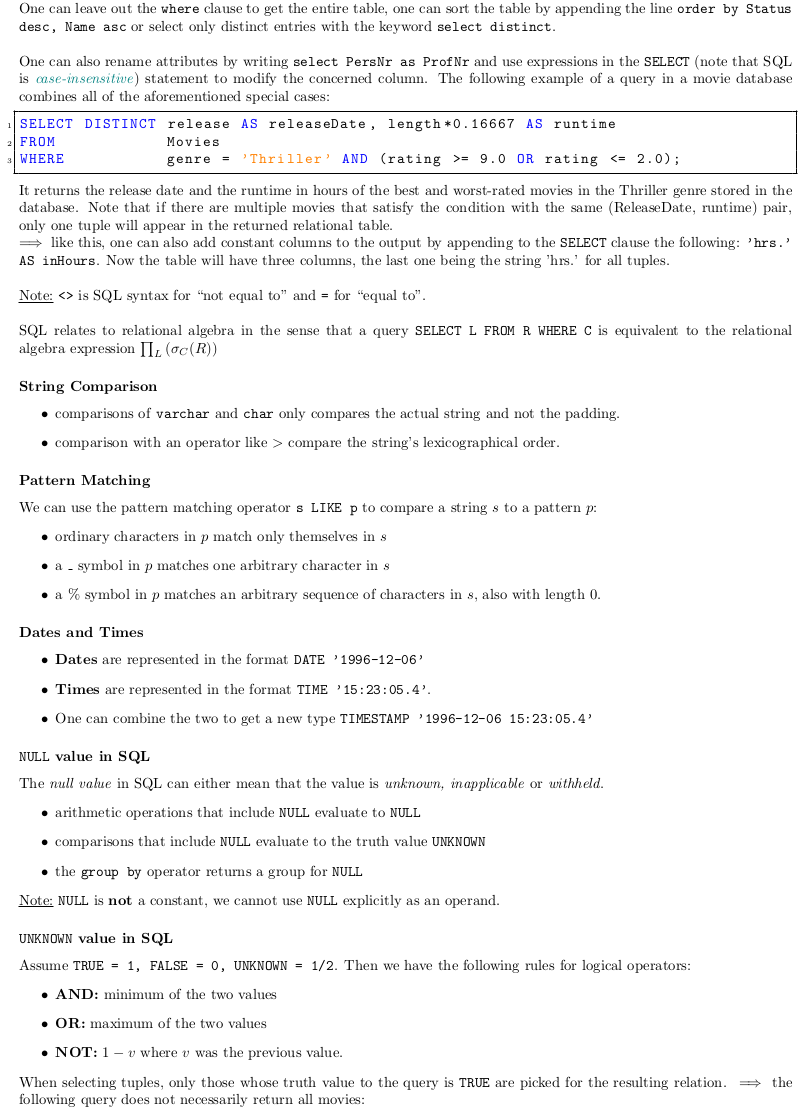
\includegraphics[width=1\linewidth]{figures/sql_4}
	\label{fig:sql4}
\end{figure}
\vspace{-\topsep}

\newpage

\vspace{-\topsep}
\begin{figure}[t!]
	\centering
	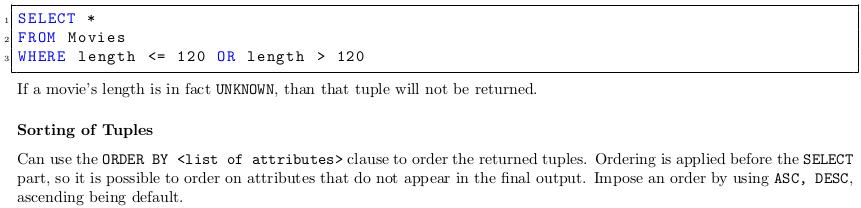
\includegraphics[width=0.95\linewidth]{figures/sql_5}
	\label{fig:sql5}
\end{figure}
\vspace{-\topsep}

\subsection{Queries on multiple Relations}

\vspace{-\topsep}
\begin{figure}[hb!]
	\centering
	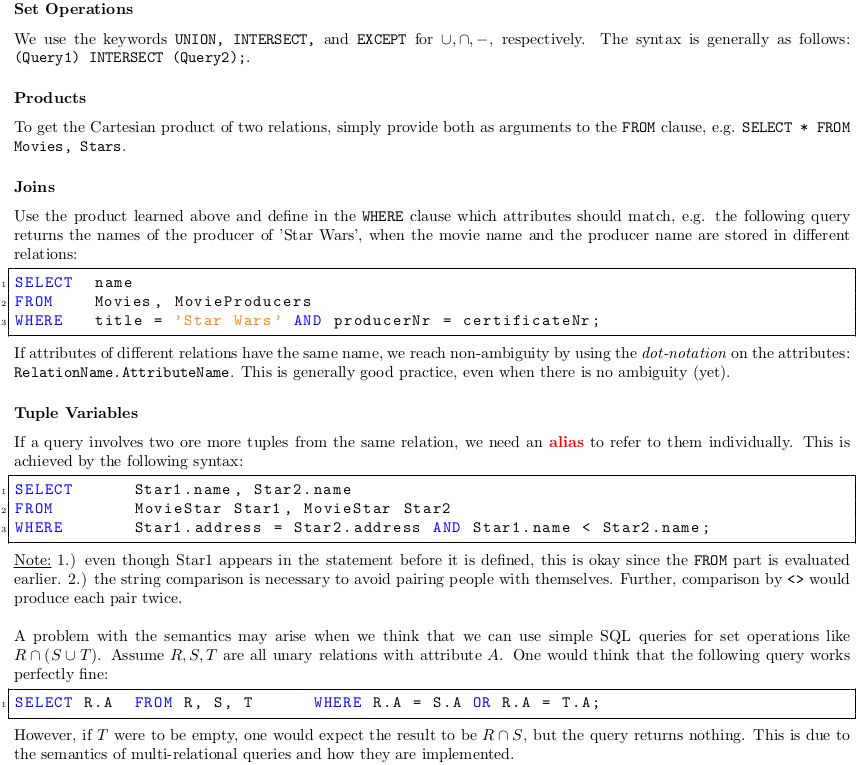
\includegraphics[width=1\linewidth]{figures/sql_6}
	\label{fig:sql6}
\end{figure}
\vspace{-\topsep}

\subsection{Full-Relation Operations}
\vspace{-\topsep}
\begin{figure}[hb!]
	\centering
	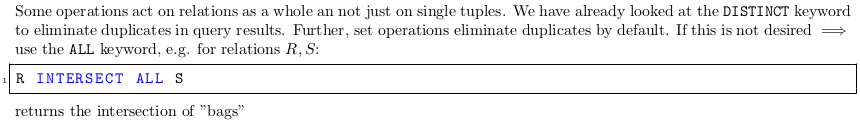
\includegraphics[width=1\linewidth]{figures/sql_7}
	\label{fig:sql7}
\end{figure}
\vspace{-\topsep}

\newpage

\vspace{-\topsep}
\begin{figure}[hb!]
	\centering
	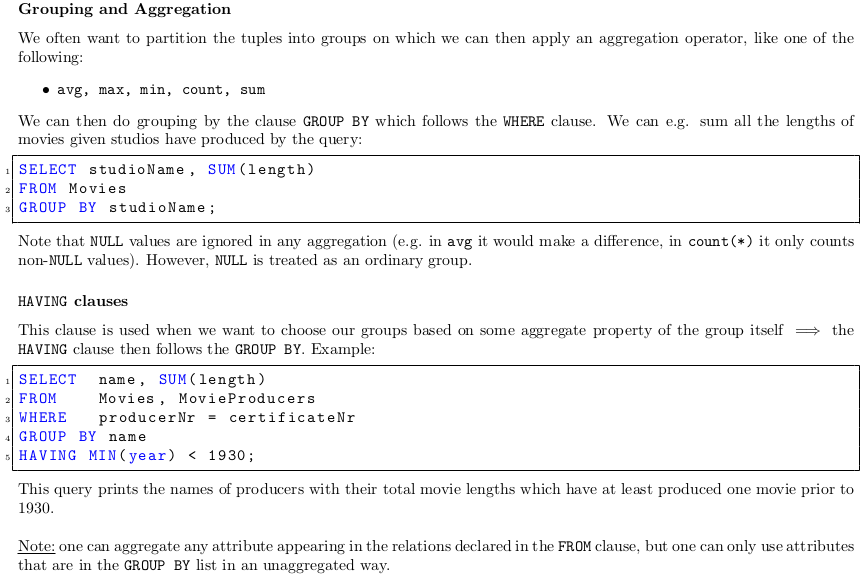
\includegraphics[width=1\linewidth]{figures/sql_8}
	\label{fig:sql8}
\end{figure}
\vspace{-\topsep}

\subsection{Subqueries}

\vspace{-\topsep}
\begin{figure}[hb!]
	\centering
	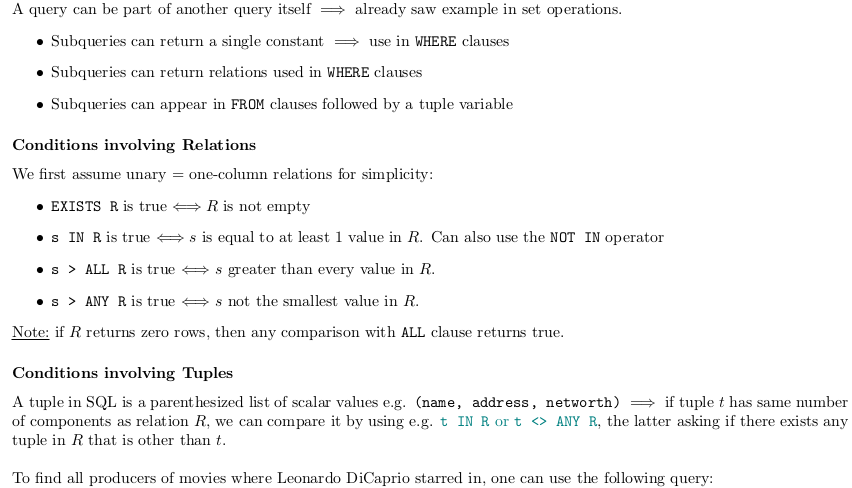
\includegraphics[width=1\linewidth]{figures/sql_9}
	\label{fig:sql9}
\end{figure}
\vspace{-\topsep}

\newpage

\vspace{-\topsep}
\begin{figure}[hb!]
	\centering
	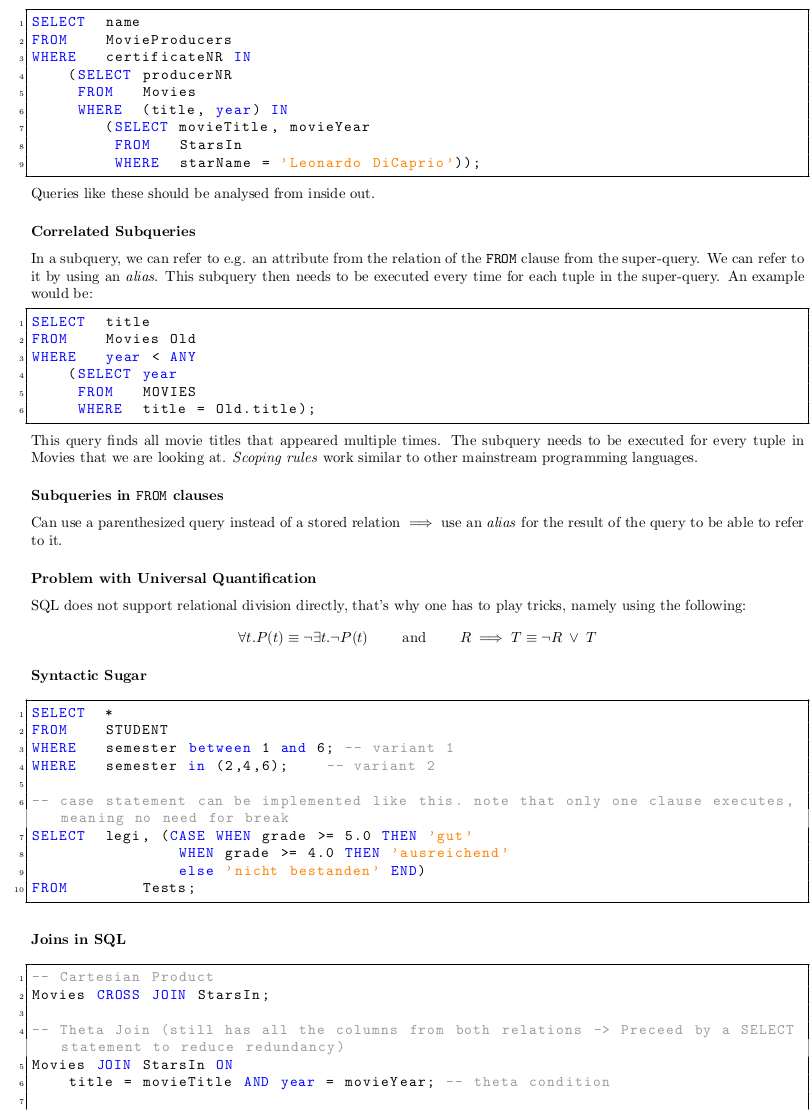
\includegraphics[width=1\linewidth]{figures/sql_10}
	\label{fig:sql10}
\end{figure}
\vspace{-\topsep}

\newpage

\vspace{-\topsep}
\begin{figure}[hb!]
	\centering
	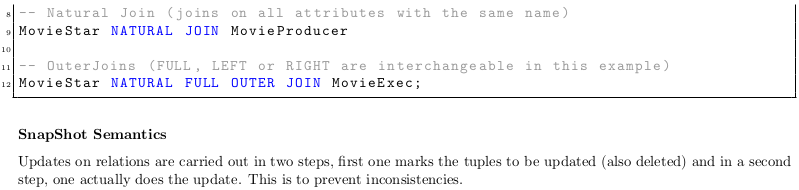
\includegraphics[width=1\linewidth]{figures/sql_11}
	\label{fig:sql11}
\end{figure}
\vspace{-\topsep}

\subsection{Views}

\vspace{-\topsep}
\begin{figure}[hb!]
	\centering
	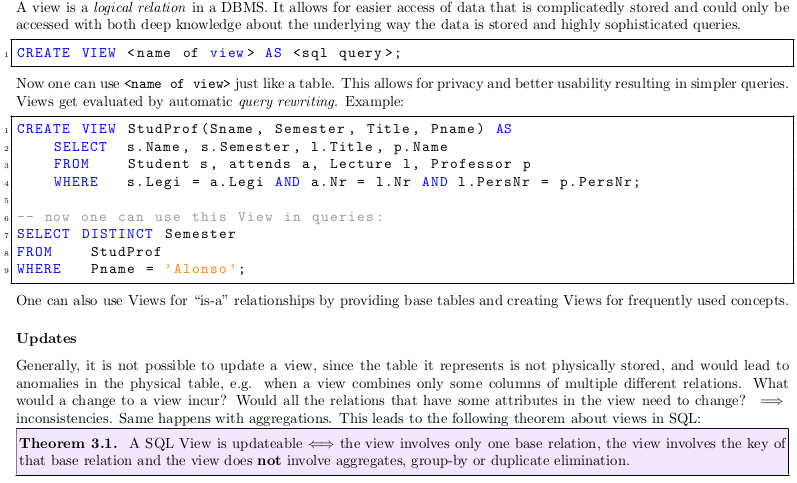
\includegraphics[width=1\linewidth]{figures/sql_12}
	\label{fig:sql12}
\end{figure}
\vspace{-\topsep}

\newpage

\section{Object Storage}

Data needs to be stored somewhere. The common notion nowadays is to just put the data in the cloud - this section describes how to do this.

As we've seen, classic relational databases that fit on a single machine are still very important today - if the data fits in a relational database, you should choose a relational database. However, petabytes of data do not fit on a single machine. We need to somehow break the monolithic relational database down and rebuild while reusing the good parts of relational databases (e.g. SQL language).\\

What can we adapt from relational databases:

\begin{compactitem}
	\item Relational algebra: selection, projection, grouping, sorting, joining
	\item Language: SQL, declarative language, functional language, optimizations, query plans, indices
	\item What is a table made of: table, rows, columns, primary key\\
\end{compactitem}

What we throw out of the window:

\begin{compactitem}
	\item Consistency constraints: Tabular integrity, Domain integrity, Atomic integrity ($1^{st}$ normal form), Boyce-Codd normal form.
	\begin{compactitem}
		\item With NoSQL, we now newly have: Heterogeneous data, Nested data, Denormalized data
	\end{compactitem}
	\item Transactions - ACID: Atomicity, Consistency, Isolation, Durability
	\begin{compactitem}
	\item With NoSQL, we now newly have: Atomic Consistency, Availability, Partition tolerance, Eventual Consistency
	\end{compactitem}
\end{compactitem}

\subsection{The stack}

\begin{figure}
	\centering
	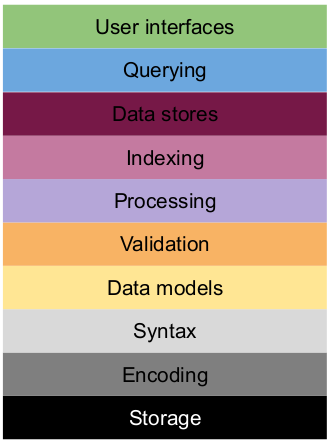
\includegraphics[width=0.2\linewidth]{figures/data_stack}
	\caption{The data stack}
	\label{fig:datastack}
\end{figure}

\begin{compactitem}
	\item \textbf{Storage} - the actual data needs to be physically stored somehow: Local filesystem, NFS, GFS, HDFS, S3, Azure Blob Storage
	\item \textbf{Encoding} - we need to somehow represent and encode data: ASCII, ISO-8859-1, UTF-8, BSON
	\item \textbf{Syntax} - represent data as text: Text, CSV, XML, JSON, RDF/XML, Turtle, XBRL
	\item \textbf{Data models} - provide a level of abstraction over the syntax (only ever dealing directly with syntax would be very tedious):	Tables (Relational model), Trees (XML Infoset, XDM), Graphs (RDF), Cubes (OLAP). All data upwards from the 'data model' level in the stack has the form of tables, trees, graphs, cubes,... \textbf{not} encoded data $\rightarrow$ level of abstraction over data.
	\item \textbf{Validation} - Check that the data is correct (e.g. check that date format is DD-MM-YYYY), data cleaning can be very expensive: XML Schema, JSON Schema, Relational schemas, XBRL taxonomies
	\item \textbf{Processing}: Two-phase processing (MapReduce), DAG-driven processing (Tez, Spark, Flink, Ray),\\ Elastic computing (EC2)
	\item \textbf{Indexing} - make processing faster by building structures: Key-value stores, Hash indices, B-Trees, Geographical indices, Spatial indices
	\item \textbf{Data stores} - the final product: RDBMS (Oracle/IBM/Microsoft), MongoDB, CouchBase, ElasticSearch, Hive, HBase, MarkLogic, Cassandra. \textbf{But} this is not yet a database, just a data store; the data store is still low level, we need a high level language for it to be a database.
	\item \textbf{Querying}: SQL, XQuery, JSONiq, N1QL, MDX, SPARQL, REST APIs
	\item \textbf{User interfaces (UI)} - user doesn't even need to use a query language: Excel,	Access,	Tableau, Qlikview, BI tools, voice assistants (Siri, Alexa,...)
\end{compactitem}

This section talks about the storage.


\subsection{Storage: from a single machine to a cluster}

Data needs to be stored somewhere. Back in the 70s, data was rather limited and we could just store databases locally on a single HDD on a single machine. In a classic file storage, files are organized in a hierarchy (the file system).\\
Typically, a file is made of:

\begin{compactitem}
	\item File metadata: information about the file such as access rights, creation date, etc. File metadata has the data shape \textit{table}.
	\item File content: The actual content is stored in blocks on disk (not just as one large junk). E.g. FFS: files are represented by inodes which point to various data blocks that make up the file.
\end{compactitem}

Issues with local storage:
\begin{compactitem}
	\item Local storage is possible on a local machine and on the LAN (e.g. a NAS). However, local storage is not usable for the WAN - we can't share a local drive with 100s of millions of people. We'd like to find a way to make this possible.
	\item Scaling issues: $10^3$ or even $10^6$ files fit on a local storage. However, we can't fit $10^9$ files on a single machine.\\
\end{compactitem}

\textbf{So how do we make this scale?}

\begin{compactitem}
	\item Use explicit block storage for better performance (expose singe blocks to users). This is not very convenient but performs better.
	\item Throw away the hierarchy and use a \textbf{flat} file system.
	\item Make metadata flexible - don't force metadata to be a table - it can be any data shape.
	\item Make the data model trivial - just assign a name to every object, i.e. an ID for each file, no more structure - essentially a \textbf{key-value store}.
	\item Use commodity hardware - scalability principle: take lots of simple, known instances (i.e. local machine).\\
\end{compactitem}

... and we get Object Storage.\\

\begin{figure}
	\centering
	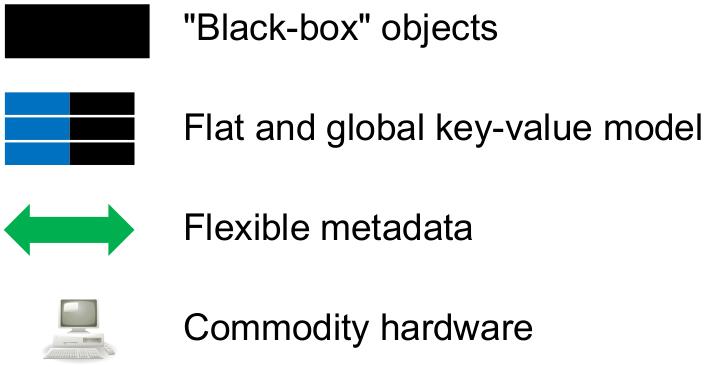
\includegraphics[width=0.25\linewidth]{figures/object_storage}
	\caption{Object storage}
	\label{fig:objectstorage}
\end{figure}

\subsection{Scale}

One single machine is not good enough - how do we scale?

\begin{compactitem}
	\item Approach 1: Scaling \textbf{UP} - more cores, more memory, etc. Scaling up gets extremely expensive very fast (exponentially) - e.g. RAM: 32GB RAM is ok, 64GB RAM is ok, 128GB is still ok, ..., 6TB RAM exists but is exponentially more expensive. 50TB RAM doesn't even exists, would need to be developed.
	\item Approach 2: Scaling \textbf{out} - instead of buying faster, bigger machines, just buy more of the same machine! Scaling up is much more scalable in terms of hardware cost - the cost essentially just increases linearly with the number of machines we buy.
	\item Approach 3: Be smart (this is the first thing you should always do)\\
\end{compactitem}

\subsection{Scaling out}

\textbf{Data centers:} All these single machines need to live somewhere - in a data center. A data center is essentially a collection of \textit{1'000 - 100'000 servers}, each of which has \textit{1-100 cores}. Having more than 100'000 servers in a single DC is hard because of coordination but mainly due to energy consumption for power and cooling. Each server has \textit{1-20TB of storage} and \textit{16GB - 6TB of RAM}. Servers are connected and the network achieves \textit{1-100 GB/s throughput} - high network throughput is very important since servers send data among each other. Servers have the form of \textit{rack servers} which allows to efficiently stack them in \textit{rack units} (RU). A DC has multiple RUs. Racks are modular - they can contain servers, storage, routers etc.\\

\textbf{Take away message: how to scale out?} Simplify the model, buy (lots of) cheap hardware, remove schemas.

\newpage

\subsection{Amazon S3}

\begin{figure}
	\centering
	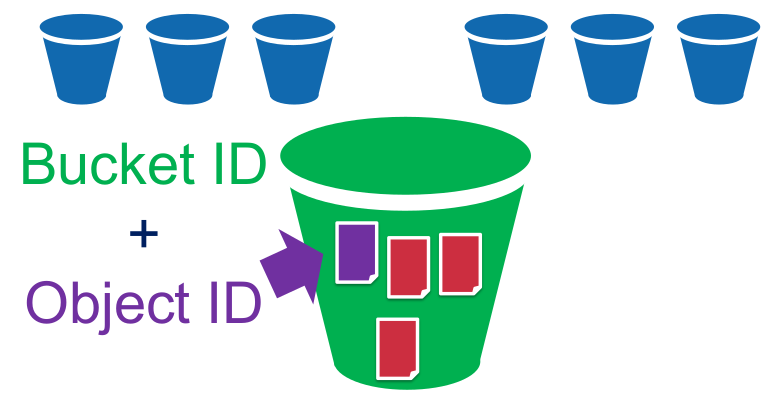
\includegraphics[width=0.2\linewidth]{figures/s3_buckets}
	\caption{S3 model}
	\label{fig:s3buckets}
\end{figure}

Amazon's S3 model is very simple, it's essentially: \textit{objects in buckets}. S3 has no tables, cubes,... and no nesting (no buckets in buckets). We have many buckets and each bucket has a \textit{bucket ID}. Each object inside a bucket has an \textit{object ID}. Having buckets makes things cleaner and makes it easy to assign them to machines. An object can be anything (picture, video, etc.) and every object can be accessed by the tuple $(bucket\_id, object\_id)$. The \textit{maximum object size is 5TB} and we can have up to 100 buckets per account (more upon request).

\textbf{Service level agreement (SLA):} SLA assures the quality of the service, e.g. 99.999999999\% durability (loss of 1 in $10^11$ objects in a year) and 99.9\% availability (1h/year downtime). Very high SLAs are \textit{very} hard to achieve (e.g. 99.99999\% SLA) corresponds to 4seconds/year outage - almost impossible. Amazon has a different approach to SLAs: response time < 10ms in 99.9\% of the cases.

\subsection{APIs}

API (application programming interface) is a set of rules and mechanisms by which one application or component interacts with the others. API can return data that you need for your application in a convenient format (e.g. JSON or XML). We need to somehow interact with the objects:

\begin{compactitem}
	\item Driver (Java Database Connectivity (JDBC)...) for various programming languages
	\item SOAP
	\item REST (lightweight version of SOAP)\\
\end{compactitem}

\subsection{Properties}

We want certain properties for databases. But:\\
\textbf{CAP theorem:} One cannot achieve consistency, availability and partition tolerance all at the same time.\\
\textit{Proof:} Imagine a system (e.g. bank) that is in a partitioned state. At right that time, someone requests the service (e.g. ATM). The system can now either serve the user - giving up partition tolerance (service will change state which won't be propagated globally due to the partition) \textit{OR} the system can not serve the user - giving up availability.

\begin{compactitem}
	\item (Atomic) Consistency:	All nodes see the same data.
	\item Availability:	It is possible to query the database at all times.
	\item Partition tolerance: The database continues to function even if the network gets partitioned.\\
\end{compactitem}

\subsection{REST APIs}

REST (representational state transfer) provides data presentation for a client in the format that is convenient for it and is typically based on the HTTP protocol. REST is not a standard or protocol, it is an approach to or architectural style for writing API! REST is based on the client-server model.

HTTP is used to request resources over a network. Resources are addressed through a URI (uniform resource identifier) e.g. \textit{http://www.ethz.ch/, http://www.mywebsite.ch/api/collection/foo/object/bar, mailto:sheldon.lee.cooper@ethz.ch}.

Let's dissect a URI: http://www.mywebsite.ch/api/collection/foo/object/bar?id=foobar\#head

\begin{compactitem}
	\item http: gives the protocol
	\item www.mywebsite.ch: the authority (domain)
	\item api/collection/foo/object/bar: the path (often this is the exact path on the server, e.g. for static websites)
	\item ?id=foobar: The query
	\item \#head: The fragment (directly jumps to specific part of the page)
\end{compactitem}

\textbf{HTTP methods}

\begin{compactitem}
	\item GET: get the resource (side-effect free)
	\item PUT: create a new resource and store it (idempotent)
	\item DELETE: delete a resource (if you send DELETE then GET on same object $\rightarrow$ 404 page not found)
	\item POST: update the corresponding resource with information provided by the client, or create this resource if it does not exist (not idempotent)\\
\end{compactitem}

All requests you make have their HTTP status codes. There are a lot of them and they are divided into 5 classes. The first number indicates which of them a code belongs to:

\begin{compactitem}
	\item 1xx - informational
	\item 2xx - success
	\item 3xx - redirection
	\item 4xx - client error
	\item 5xx - server error
\end{compactitem}


\subsubsection{S3}

REST with S3: buckets and objects: http://\textit{bucket}.s3.amazonaws.com/\textit{object-name}

\textbf{S3 REST API:}

\begin{compactitem}
	\item Bucket: \{PUT, DELETE, GET\} bucket
	\item Object: \{PUT, DELETE, GET\} object\\
\end{compactitem}

\textbf{Folders: is S3 a file system?}
The physical file system in S3 is flat - there are no folders/hierarchies. But we can simulate a hierarchy by naming objects as if they were in a hierarchy. This will be displayed as a hierarchy. Thus, on the logical level (browsing), S3 looks like a hierarchical file system but on the physical level (object keys) it's really a flat file system. (Again, it is important to distinguish between the physical and logical part).\\
The objects would then have names such as \textit{/food/fruits/orange, /food/vegetables/tomato} which simulates the hierarchy.

S3 can host various things such as static websites or datasets. Datasets are just lots different files put into objects. This is different from relational DBs where we split data by having different tables for different instances (e.g. order, customer table). Here we don't have a file for order and a file for customer.\\

\subsection{More on storage}

\textbf{Replication}: We want fault tolerance (faults happen). This can be achieved by replication (if you replicate the file, loosing it totally is less likely). Faults can happen locally (node failure) and regionally (natural catastrophe).
\begin{compactitem}
	\item Local fault: replicate over multiple local machines
	\item Regional fault: replicate over multiple DCs in various regions. This gives us better resiliency to natural catastrophes and better latency.
\end{compactitem}

Cloud providers offer different storage classes, trading availability for cost:

\begin{compactitem}
	\item Standard: High availability
	\item Standard - Infrequent Access: Less availability, Cheaper storage, Cost for retrieving
	\item Amazon Glacier: Low-cost, Hours to GET\\
\end{compactitem}

\subsection{Azure Blob Storage}

Azure blob storage is different from S3:

\begin{tabular}{|c|c|c|}
	\hline 
	& S3 & Azure \\ 
	\hline 
	Object ID & Bucket + Object & Account + Container + Blob \\ 
	\hline 
	Object API & Blackbox & Block (like bucket)/Append (for logs)/Page (for VMs)\\ 
	\hline 
	Limit & 5TB & 4.78 TB (block), 195 GB (append),	8TB (page) \\ 
	\hline
\end{tabular}\\

Azure thus has one more layer of indirection: account, container, blob. Further, Azure doesn't view an object as a blackbox, it let's you see inside and differentiate between 3 types of blobs: block, append, page. The account name maps to a virtual machine which is responsible for my data. The partition name is a chunk of data and the stream layer streams data over to me. In the Azure datacenter (i.e. one storage stamp) we have 10-20 racks, each with 18 storage nodes. This totals to 30PB ($= 30*10^{15} bytes$) per datacenter - over the whole world, Azure reaches an exabyte range of storage. Azure keeps the usage of the datacenter below 70-80\% storage capacity since dealing with full storage is annoying.\\

\textbf{Storage replication:}

\begin{compactitem}
	\item Intra-stamp replication (synchronous): Replication within the streaming later (i.e. within the same location (data center)).
	\item Inter-stamp replication (asynchronous): Replication between different partition layers (i.e. between different locations (data centers))\\
\end{compactitem}

\textbf{Location services:} Azure has globally distributed data centers for load balancing and latency optimization. The location service works as follows:

\begin{compactenum}
	\item Location service sends request with account name to DNS server.
	\item DNS server returns a virtual IP that is mapped to the account name. The virtual IP points to a primary storage stamp and also to a backup storage stamp.
\end{compactenum}

\vspace{-\topsep}
\begin{figure}[hb!]
	\centering
	\begin{subfigure}[t]{.5\textwidth}
		\centering
		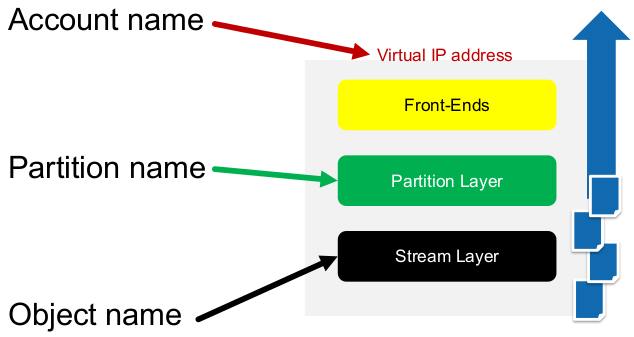
\includegraphics[width=0.5\linewidth]{figures/azure_storage_stamp}
		\caption{Azure storage stamp}
		\label{fig:azure_storage_stamp}
	\end{subfigure}%
	\begin{subfigure}[t]{.5\textwidth}
		\centering
		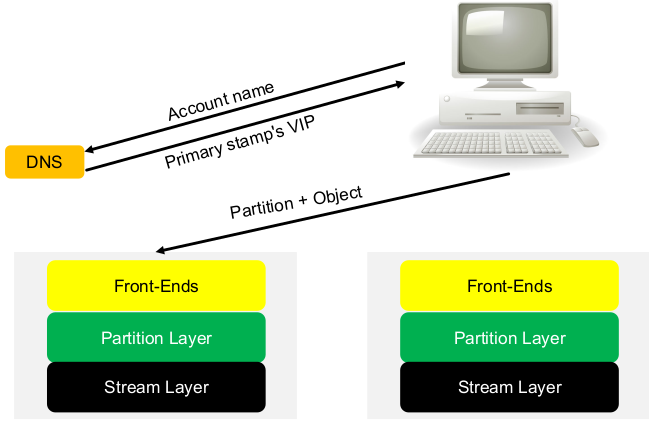
\includegraphics[width=0.6\linewidth]{figures/azure_location_services}
		\caption{Azure location services}
		\label{fig:azure_location_services}
	\end{subfigure}
\end{figure}

\subsection{Mindsets}

Amazon and Azure have different mindsets in their cloud services:

\begin{compactitem}
	\item Amazon mindset: Amazon thinks a lot in terms of modules. They have ~200 different services they offer (S3, domain management, AWS,...) $\rightarrow$ a lot of small services that each do one particular thing.
	\item Azure mindset: Azure has bigger services that do more $\rightarrow$ fewer services that do several things.
\end{compactitem}

\section{Distributed file systems}

Where does data come from?

\begin{compactitem}
	\item Raw data: sensors, measurements, events, logs (e.g. CERN sensor measurements)
	\item Derived data: aggregated data, intermediate data (e.g. computational results on sensor measurements)
\end{compactitem}

Big Data isn't big data - there are different cases:

\begin{compactitem}
	\item \textbf{A	huge amount of large files} (billions of TB files): This is what S3 is $\rightarrow$ lots of files, but single files are not extremely big, just large (e.g. 5TB for S3).\\
	$\rightarrow$ Object storage + Key-value model
	\item \textbf{A large amount of huge files} (millions of PB files): We need something new for this...\\
	$\rightarrow$ Block storage + file system
\end{compactitem}

Google had just this idea: have a FS that looks and feels like a normal file system \textit{but} lives on a distributed cluster. Google went on and developed GoogleFS.

\subsection{Fault tolerance and robustness}

We have different paradigms for fault tolerance:

\begin{compactitem}
	\item Local disk: the disk \textit{might} fail, we can just keep a backup \textit{in case.}
	\item Cluster with 100s to 10'000s machines: nodes \textit{will} fail ($P[\text{at least one node fails
	}] = 1-(1-p)^n$, with $n$: \#nodes, $p$: failure probability of a single node). We thus need a stronger property for clusters, we can't restore from backups every single day.
\end{compactitem}

How to achieve fault tolerance and robustness on clusters:

\begin{compactitem}
	\item Fault tolerance (system keeps working under faults)
	\item Automatic Recovery (can't recover manually with lots of disks)
	\item Error detection (know about failed disks)
	\item Monitoring (keep an overview over what's working)
\end{compactitem}

\subsection{File system specifications}

\textbf{File read/update model:}

\begin{compactitem}
	\item Random access (can read at any position in a file): this is hard to do in clusters
	\item Sequential access (scan the file from the beginning (reading)/ append to file (update): this is easier for distributed clusters, that's why (most) do it like this
\end{compactitem}

Appends: You can only append, can't go back and change something. This is suitable for sensor data, logs and also intermediate data. \textbf{Note:} Since we have a distributed FS, we have 100s of clients in parallel reading/writing $\rightarrow$ we want atomicity.

\textbf{Performance requirements:}

Our top priority is throughput (how fast do you read/write). Secondary, we want latency (time until we start reading/writing).

Remember: we have a huge discrepancy between storage capacity, throughput and latency. Over the last 60 years, storage capacity improved by 200'000'000'000, throughput improved by 10'000 and latency improved by 8. The solution for the capacity-throughput discrepancy is to parallelize. The solution for the throughput-latency discrepancy is to do batch-processing.\\
Latency is usually not a problem in big data since the data is so large, the read/write time dominates the latency.\\
A similar discrepancy between throughput and latency can be observed in websites. In the 90s, a website started loading slowly, elements appeared one after another $\rightarrow$ throughput was the issue. Today, website is blank for ~1s and then the whole website appears $\rightarrow$ latency is the issue.

\subsection{Hadoop}

Hadoop is primarily:

\begin{compactitem}
	\item Distributed File System (HDFS) (inspired by Google's GFS)
	\item MapReduce (inspired by Google's MapReduce)
	\item Wide column store (HBase) (inspired by Google's BigTable)
\end{compactitem}

\subsection{Distributed file systems: the model}

Again, rememeber data independence: separate the logical model from the physical model.

\textbf{File system (logical model):} In distributed file systems, we have a \textbf{file hierarchy} (unlike the key-value model in object storage which is flat).

\textbf{Block storage (physical storage):} In distributed file systems, we have block storage (unlike object storage where we have a blackbox model). Terminology: HDFS: Block, GFS: Chunk.
We thus have a hierarchy of files where each file is associated with a chain of blocks.\\

Why blocks? 1) The files are bigger than a disk (PBs) , there is no way the files fit on a single machine $\rightarrow$ need blocks. 2) Simple level of abstraction.

\textbf{Block size:} Every file is a multiple of blocks. In a simple file system, we have a block size of 4kB $\rightarrow$ good size for local machines, good compromise. However, in distributed file systems, things are different: blocks travel over the network and we have very large (PB) files. Due to the throughput-latency discrepancy, we want larger blocks (for small blocks, the latency would outweigh the transfer time). Further, large blocks lead to less blocks being read per file. The block size in distributed file systems is \textbf{64MB - 128MB}. This is a good compromise - not too many blocks for big files, but also small enough to have several blocks on one machine.\\

\subsection{HDFS Architecture}

\begin{figure}[hb!]
	\centering
	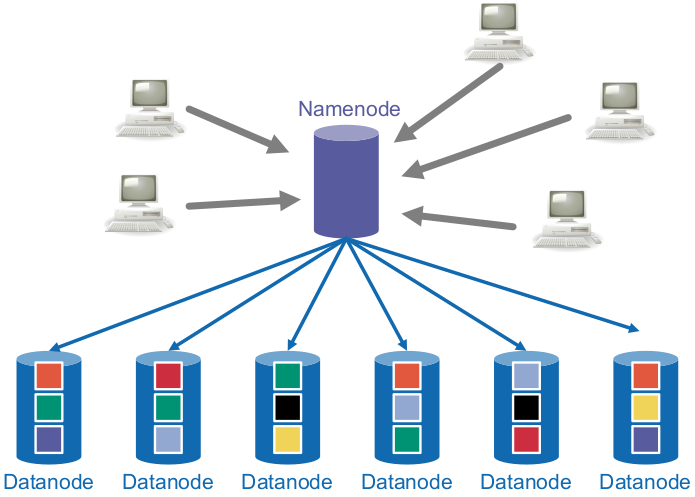
\includegraphics[width=0.3\linewidth]{figures/hdfs_architecture}
	\label{fig:hdfsarchitecture}
\end{figure}


We need to connect the many machines somehow. One possible way would be peer-to-peer, but this is not ideal. HDFS uses a master-slave architecture: the namenode (has the names of the files) is the master and the datanodes (have the actual data) are the slaves.\\
How it works from the file perspective: The file is divided into 128MB chunks. The chunks are then stored in datanodes. Each chunk is replicated 3 times (the \# of replicas can be specified).

\subsubsection{Namenode}

The namenode will be concurrently accessed by multiple clients. The namenode is responsible for all system-wide activity:

\begin{compactitem}
	\item File namespace (+Access Control): keep track of hierarchy of files. This is actually rather small (hierarchy doesn't contain the actual file data, just the hierarchy).
	\item File to block mapping: every file is associated with a list of blocks. The namenode keeps track of the mapping $file \rightarrow \{blocks\}$.
	\item Block location: for every block, the namenode needs to know on which 3 (default) datanodes the block is stored.
\end{compactitem}

\subsubsection{Datanode}

A datanode is a machine with multiple local disks. Blocks are stored on these local disks. Datanodes are responsible for failure detection. Each datanode has its own local view over its disks - proximity to hardware facilitates disk failure detection. Each block has a \textit{block ID (64bit)}. It is also possible to access blocks at a subblock granularity to request parts of a block.

\subsubsection{Communication}

\textbf{Client protocol:} The client protocol handles \textit{client-namenode} communication. Clients sends metadata operations (e.g. create directory, delete directory, write file, append to file, read file,
delete file) and the namenode responds with the datanode location and the block IDs.\\

\textbf{DataNode protocol:} The datanode protocol handles \textit{datanode-namenode} communication. The datanode always initiates the connection. The following types of datanode-namenode communication exist:

\begin{compactitem}
	\item registration
	\item heartbeat: datanode tells namenode every 3s that it's still alive
	\item blockreport: every 6h, datanode sends full list of blocks (not the contents of the blocks) to the namenode
	\item blockreceived\\
\end{compactitem}

\textbf{Data transfer protocol:} The data transfer protocol handles \textit{client-datanode} communication and is used by clients to read actual block content. The client knows which datanode to contact for a given block - it got that information from the namenode.\\
Client reads a file:

\begin{compactenum}
	\item Client asks namenode for file
	\item Namenode sends block location (multiple datanodes for each block, sorted by distance) to client
	\item Client reads data from datanode via input stream\\
\end{compactenum}

Client writes a file:

\begin{compactenum}
	\item Client sends create to namenode
	\item Namenode sends datanodes for first block
	\item Client organizes pipeline by contacting one datanode and tells the datanode which other datanodes to forward the data to
	\item Client then sends the data over to the datanode
	\item Datanode sends Ack
	\item Namenode sends datanodes for second block (writing happens block by block, for every block the client contacts a datanode which will also forward to other datanodes (note: if the blocks were very small, this would have large overhead))
	\item ...
	\item Client sends close/release lock
	\item Datanodes check with namenode for minimal replication (datanode protocol)
	\item Namenode sends Ack to client
	\item Namenode replicates further asynchronously
\end{compactenum}

This block-by-block writing is all done simultaneously under DFSOutputStream (streaming through), checksums are used to provide data integrity.

\begin{figure}[hb!]
	\centering
	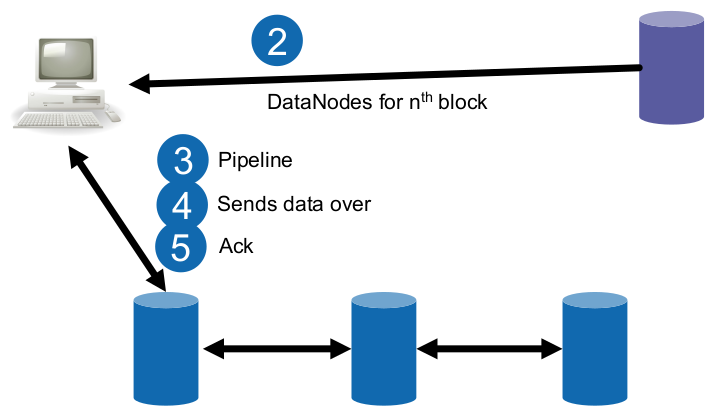
\includegraphics[width=0.4\linewidth]{figures/hdfs_client_write}
	\label{fig:hdfsclientwrite}
\end{figure}

\newpage

\subsection{Replicas}

The number of replicas per file can be specified (default: 3). The replicas need to be placed in a smart way. Have the topology of a data center in mind: we have a cluster consisting of multiple racks, each rack consisting of multiple nodes. We add a notion of distance between nodes $D(A,B)$.\\
The replicas are placed as follows:

\begin{compactitem}
	\item Replica 1: same node as client (or random), rack A\\
	(Note: in practice, the actual client is not on my laptop but on a node in the data center and my laptop connects to it. The 1st replica goes on that node because it's very efficient).
	\item Replica 2: a node in a different rack B (put in a different rack from 1st replica - racks can fail)
	\item Replica 3: in same rack B but on a different node
	\item Replica 4 and beyond: random, but if possible:
	\begin{compactitem}
		\item at most one replica per node
		\item at most two replicas per rack\\
	\end{compactitem}
\end{compactitem}

What if we placed replicas 1\&2 on the same rack? If you always put the first two replicas on the same rack as my client node $\rightarrow$ 2/3 of replicas of all blocks written by the client will be on the same rack (the client stays on the same node) $\rightarrow$ worse replication factor.\\

We could also put all first 3 replicas on 3 different racks, but this would need more data being sent between racks (takes longer).

\subsection{Performance and availability}

The NameNode is responsible for file namespace, file-block mapping, block locations and is a single point of failure. We want the file namespace and file-block mapping to persist. HDFS thus puts the namespace file and an edit log onto persistent storage (edit log allows to not rebackup the whole hierarchy and mapping, only the things that change). We further also backup the persistent storage with the namespace file and the edit log to shared drives/ backup drives/ etc.\\

What if the namenode fails? We need to start it up again:

\begin{compactitem}
	\item Restore the initial hierarchy/ block mapping and then 'play' the edit log and apply changes to the file systems (restore last logged version)
	\item Receive the block locations from the block reports, which are periodically sent by the datanode (can also be manually requested)
\end{compactitem}

This startup takes ~30min. Can we do better?

\begin{compactitem}
	\item Checkpoints: periodically play the edit log and reconstruct a more recent namespace file. This way, we don't have to replay the \textit{whole} edit log upon failure.
	\item High Availability (HA): Standby NameNodes. Have standby machines that keep the exact same state and immediately take over in case the active namenode crashes.
	\item Federated DFS
\end{compactitem}

\subsection{Using HDFS}





\titlespacing{\subsection}{0pt}{2ex}{2ex}

\label{lastpage} % this must stay here
\clearpage
\addcontentsline{toc}{section}{References}
\bibliographystyle{acm}
\bibliography{refs}

\clearpage
\appendix
\pagenumbering{Roman}

\end{document}
